\documentclass[utf8x, 12pt]{G7-32}

% Настройки стиля ГОСТ 7-32
% Для начала определяем, хотим мы или нет, чтобы рисунки и таблицы нумеровались в пределах раздела, или нам нужна сквозная нумерация.
\EqInChapter % формулы будут нумероваться в пределах раздела
\TableInChapter % таблицы будут нумероваться в пределах раздела
\PicInChapter % рисунки будут нумероваться в пределах раздела
\usepackage{slashbox}

\usepackage[table,xcdraw]{xcolor}

% Добавляем гипертекстовое оглавление в PDF
\usepackage[
bookmarks=true, colorlinks=true, unicode=true,
urlcolor=black,linkcolor=black, anchorcolor=black,
citecolor=black, menucolor=black, filecolor=black,
]{hyperref}

% Изменение начертания шрифта --- после чего выглядит таймсоподобно.
% \usepackage{cyrtimespatched}

% графика
\usepackage{graphicx}
\graphicspath{ {./img/} }

% отделять первую строку раздела абзацным отступом
\usepackage{indentfirst} 

% Пакет Tikz
\usepackage{tikz}
\usetikzlibrary{arrows,positioning,shadows}

% Произвольная нумерация списков.
\usepackage{enumerate}

% ячейки в несколько строчек
\usepackage{multirow}

% itemize внутри tabular
\usepackage{paralist,array}

% объявляем новую команду для переноса строки внутри ячейки таблицы
\newcommand{\specialcell}[2][c]{%
	\begin{tabular}[#1]{@{}c@{}}#2\end{tabular}}

\usepackage{tikz}
\usepackage{pgfplots}
\usepackage{pdfpages}
\usepackage{caption}
\usepackage{longtable}
% \captionsetup[table]{position=top}
% Листинги

\usepackage{listings}
\usepackage{caption}

\usepackage{courier}
\usepackage{wrapfig}

\usepackage{xcolor}
\captionsetup[lstlisting]{singlelinecheck=off, justification=raggedright}


\definecolor{codegreen}{rgb}{0,0.6,0}
\definecolor{codegray}{rgb}{0.5,0.5,0.5}
\definecolor{codepurple}{rgb}{0.58,0,0.82}
\definecolor{backcolour}{rgb}{0.95,0.95,0.92}


% Значения по умолчанию
\lstset{
  % подсветка синтаксиса
  backgroundcolor=\color{backcolour},   
  commentstyle=\color{codegreen},
  keywordstyle=\color{magenta},
  numberstyle=\tiny\color{codegray},
  stringstyle=\color{codepurple},
  basicstyle= \footnotesize,
  breakatwhitespace=true,% разрыв строк только на whitespacce
  breaklines=true,       % переносить длинные строки
%   captionpos=b,          % подписи снизу -- вроде не надо
  inputencoding=koi8-r,
  numbers=left,          % нумерация слева
  numberstyle=\footnotesize,
  showspaces=false,      % показывать пробелы подчеркиваниями -- идиотизм 70-х годов
  showstringspaces=false,
  showtabs=false,        % и табы тоже
  stepnumber=1,
  tabsize=4,              % кому нужны табы по 8 символов?
  frame=single,
  escapeinside={(*}{*)}, %выделение
  literate={а}{{\selectfont\char224}}1
  {б}{{\selectfont\char225}}1
  {в}{{\selectfont\char226}}1
  {г}{{\selectfont\char227}}1
  {д}{{\selectfont\char228}}1
  {е}{{\selectfont\char229}}1
  {ё}{{\"e}}1
  {ж}{{\selectfont\char230}}1
  {з}{{\selectfont\char231}}1
  {и}{{\selectfont\char232}}1
  {й}{{\selectfont\char233}}1
  {к}{{\selectfont\char234}}1
  {л}{{\selectfont\char235}}1
  {м}{{\selectfont\char236}}1
  {н}{{\selectfont\char237}}1
  {о}{{\selectfont\char238}}1
  {п}{{\selectfont\char239}}1
  {р}{{\selectfont\char240}}1
  {с}{{\selectfont\char241}}1
  {т}{{\selectfont\char242}}1
  {у}{{\selectfont\char243}}1
  {ф}{{\selectfont\char244}}1
  {х}{{\selectfont\char245}}1
  {ц}{{\selectfont\char246}}1
  {ч}{{\selectfont\char247}}1
  {ш}{{\selectfont\char248}}1
  {щ}{{\selectfont\char249}}1
  {ъ}{{\selectfont\char250}}1
  {ы}{{\selectfont\char251}}1
  {ь}{{\selectfont\char252}}1
  {э}{{\selectfont\char253}}1
  {ю}{{\selectfont\char254}}1
  {я}{{\selectfont\char255}}1
  {А}{{\selectfont\char192}}1
  {Б}{{\selectfont\char193}}1
  {В}{{\selectfont\char194}}1
  {Г}{{\selectfont\char195}}1
  {Д}{{\selectfont\char196}}1
  {Е}{{\selectfont\char197}}1
  {Ё}{{\"E}}1
  {Ж}{{\selectfont\char198}}1
  {З}{{\selectfont\char199}}1
  {И}{{\selectfont\char200}}1
  {Й}{{\selectfont\char201}}1
  {К}{{\selectfont\char202}}1
  {Л}{{\selectfont\char203}}1
  {М}{{\selectfont\char204}}1
  {Н}{{\selectfont\char205}}1
  {О}{{\selectfont\char206}}1
  {П}{{\selectfont\char207}}1
  {Р}{{\selectfont\char208}}1
  {С}{{\selectfont\char209}}1
  {Т}{{\selectfont\char210}}1
  {У}{{\selectfont\char211}}1
  {Ф}{{\selectfont\char212}}1
  {Х}{{\selectfont\char213}}1
  {Ц}{{\selectfont\char214}}1
  {Ч}{{\selectfont\char215}}1
  {Ш}{{\selectfont\char216}}1
  {Щ}{{\selectfont\char217}}1
  {Ъ}{{\selectfont\char218}}1
  {Ы}{{\selectfont\char219}}1
  {Ь}{{\selectfont\char220}}1
  {Э}{{\selectfont\char221}}1
  {Ю}{{\selectfont\char222}}1
  {Я}{{\selectfont\char223}}1
}

\lstloadlanguages{
  C++
}

% Стиль для псевдокода: строчки обычно короткие, поэтому размер шрифта побольше
\lstdefinestyle{pseudocode}{
  basicstyle=\small,
  keywordstyle=\color{black}\bfseries\underbar,
  language=Pseudocode,
  numberstyle=\footnotesize,
  commentstyle=\footnotesize\it
}

% Стиль для обычного кода: маленький шрифт
\lstdefinestyle{realcode}{
  basicstyle=\scriptsize,
  numberstyle=\footnotesize
}

% Стиль для коротких кусков обычного кода: средний шрифт
\lstdefinestyle{simplecode}{
  basicstyle=\footnotesize,
  numberstyle=\footnotesize
}

% Стиль для BNF
\lstdefinestyle{grammar}{
  basicstyle=\footnotesize,
  numberstyle=\footnotesize,
  stringstyle=\bfseries\ttfamily,
  language=BNF
}

% Определим свой язык для написания псевдокодов на основе Python
\lstdefinelanguage[]{Pseudocode}[]{Python}{
  morekeywords={each,empty,wait,do},% ключевые слова добавлять сюда
  morecomment=[s]{\{}{\}},% комменты {а-ля Pascal} смотрятся нагляднее
  literate=% а сюда добавлять операторы, которые хотите отображать как мат. символы
    {->}{\ensuremath{$\rightarrow$}~}2%
    {<-}{\ensuremath{$\leftarrow$}~}2%
    {:=}{\ensuremath{$\leftarrow$}~}2%
    {<--}{\ensuremath{$\Longleftarrow$}~}2%
}[keywords,comments]

% Свой язык для задания грамматик в BNF
\lstdefinelanguage[]{BNF}[]{}{
  morekeywords={},
  morecomment=[s]{@}{@},
  morestring=[b]",%
  literate=%
    {->}{\ensuremath{$\rightarrow$}~}2%
    {*}{\ensuremath{$^*$}~}2%
    {+}{\ensuremath{$^+$}~}2%
    {|}{\ensuremath{$|$}~}2%
}[keywords,comments,strings]

% Подписи к листингам на русском языке.
\renewcommand\lstlistingname{\cyr\CYRL\cyri\cyrs\cyrt\cyri\cyrn\cyrg}
\renewcommand\lstlistlistingname{\cyr\CYRL\cyri\cyrs\cyrt\cyri\cyrn\cyrg\cyri}



\begin{document}

\frontmatter % выключает нумерацию ВСЕГО; здесь начинаются ненумерованные главы: реферат, введение, глоссарий, сокращения и прочее.
\begin{table}[ht]
	\centering
	\begin{tabular}{|c|p{400pt}|} 
	\hline
		\begin{tabular}[c]{@{}c@{}} 
\includegraphics[scale=0.37]{EmblemBMSTU} \\\end{tabular} &
		\footnotesize\begin{tabular}[c]{@{}c@{}}\textbf{Министерство~науки~и~высшего~образования~Российской~Федерации}\\\textbf{Федеральное~государственное~бюджетное~образовательное~учреждение}\\\textbf{~высшего~образования}\\\textbf{«Московский~государственный~технический~университет}\\\textbf{имени~Н.Э.~Баумана}\\\textbf{(национальный~исследовательский~университет)»}\\\textbf{(МГТУ~им.~Н.Э.~Баумана)}\\\end{tabular}  \\
	\hline
	\end{tabular}
\end{table}
\noindent\rule{\textwidth}{4pt}
\noindent\rule[14pt]{\textwidth}{1pt}
\hfill 
\noindent
\makebox{ФАКУЛЬТЕТ~}%
\makebox[\textwidth][l]{\underline{~~~~«Информатика и системы управления»~~~~~~~~~~~~~~~~~~~~~~~~~~~~~~~~~~~~~~~~~~~~}}%
\\
\noindent
\makebox{КАФЕДРА~}%
\makebox[\textwidth][l]{\underline{~~~~~~~«Программное обеспечение ЭВМ и информационные технологии»~~~~~~~~}}%
\\


\begin{center}
	\vspace{3cm}
	{\bf\huge Отчёт\par}
	{\bf\Large по лабораторной работе №2\par}
	\vspace{0.5cm}
\end{center}


\noindent
\makebox{\large{\bf Название:}~~~}
\makebox[\textwidth][l]{\large\underline{~Алгоритм Винограда~~~~~~~~~~~~~~~~~~~~~~~~~~~~~~~~~~~~~~~~~~~~~~~~~~~~~~}}\\

\noindent
\makebox{\large{\bf Дисциплина:}~~~}
\makebox[\textwidth][l]{\large\underline{~Анализ алгоритмов~~~~~~~~~~~~~~~~~~~~~~~~~~~~~~~~~~~~~~~~~~~~~~~~~~~~}}\\

\vspace{1.5cm}
\noindent
\begin{tabular}{l c c c c c}
    Студент      & ~ИУ7-55Б~               & \hspace{3.5cm} & \hspace{3.5cm}                 & &  И. Е. Афимин \\\cline{2-2}\cline{4-4} \cline{6-6} 
    \hspace{3cm} & {\footnotesize(Группа)} &                & {\footnotesize(Подпись, дата)} & & {\footnotesize(И.О. Фамилия)}
\end{tabular}

\vspace{1cm}

\noindent
\begin{tabular}{l c c c c}
    Преподаватель & \hspace{6cm}   & \hspace{3.5cm}                 & & Л.Л. Волкова \\\cline{3-3} \cline{5-5} 
    \hspace{3cm}  &                & {\footnotesize(Подпись, дата)} & & {\footnotesize(И.О. Фамилия)}
\end{tabular}

\begin{center}	
	\vfill
	\large \textit {Москва, 2020}
\end{center}

\thispagestyle {empty}
\pagebreak

\tableofcontents

\newpage
\chapter*{Введение}
\addcontentsline{toc}{chapter}{Введение}
\textbf{Цель работы:} изучение алгоритмов умножения матриц. В данной лабораторной работе рассматривается стандартный алгоритм умножения матриц, алгоритм Винограда и модифицированный алгоритм Винограда.  Также требуется изучить рассчет сложности алгоритмов, получить навыки в улучшении алгоритмов.

Задачами данной лабораторной являются:
\begin{enumerate}
  	\item изучить алгоритмы умножения матриц: стандартный и алгоритм Винограда; 
	\item оптимизировать алгоритм Винограда;
	\item дать теоретическую оценку базового алгоритма умножения матриц, алгоритма Винограда и улучшенного алгоритма Винограда;
	\item реализовать три алгоритма умножения матриц на одном из языков программирования;
	\item сравнить алгоритмы умножения матриц.
\end{enumerate}

\mainmatter % это включает нумерацию глав и секций в документе ниже
\chapter{Аналитическая часть}
В данном разделе рассмотрим понятие произведения матриц, классическое произведение и произведение матриц при помощи алгоритма Винограда
\section{Умножение матриц}
Матрицей A размера $[m*n]$ называется прямоугольная таблица
чисел, функций или алгебраических выражений, содержащая m строк и n столбцов. Числа m и n определяют размер матрицы. Если число столбцов в первой матрице совпадает с числом строк во второй, то эти две матрицы можно перемножить. У произведения будет столько же строк, сколько в первой матрице, и столько же столбцов, сколько во второй \cite{link3}.
	    
Пусть даны две прямоугольные матрицы А и В размеров $[m * n]$ и $[n * k]$ соответственно.  
В результате произведение матриц A и B получим матрицу C размера $[m *  k]$.


$c_{i,j} = \sum\limits_{r=1}^n a_{i,r}\cdot b_{r,j}$ называется произведением матриц A и B.

\section{Алгоритм Винограда}
Подход Алгоритма Винограда является иллюстрацией общей методологии, начатой в 1979-х годах на основе
билинейных и трилинейных форм, благодаря которым большинство усовершенствований для умножения матриц были получены.

Рассмотрим два вектора $V = (v1, v2, v3, v4)$ и $W = (w1, w2, w3, w4)$.  

 Их скалярное произведение равно (\ref{formula}) 

\begin{equation} \label{formula}
V \cdot W=v_1 \cdot w_1 + v_2 \cdot w_2 + v_3 \cdot w_3 + v_4 \cdot w_4
\end{equation}

Равенство (\ref{formula}) можно переписать в виде (\ref{formula2}) 
\begin{equation} \label{formula2}
V \cdot W=(v_1 + w_2) \cdot (v_2 + w_1) + (v_3 + w_4) \cdot (v_4 + w_3) - v_1 \cdot v_2 - v_3 \cdot v_4 - w_1 \cdot w_2 - w_3 \cdot w_4
\end{equation}

Выражение в правой части последнего равенства допускает предварительную обработку: его части можно вычислить заранее и запомнить для каждой строки первой матрицы и для каждого столбца второй. 
Это означает, что над предварительно обработанными элементами нам придется выполнять лишь первые два умножения и последующие пять сложений, а также дополнительно два сложения. 

\section{Вывод}
Были рассмотрены алгоритмы классического умножения матриц и алгоритм Винограда, основное отличие которых — наличие предварительной обработки, а также количество операций умножения.




\chapter{Конструкторская часть}
    В данном разделе будут рассмотрены требования к функциональности ПО, схемы алгоритмов
    и определены способы тестирования.

    \section{Требования к функциональности ПО}
        В данной работе требуется обеспечить следующую минимальную функциональность консольного приложения.
            \begin{enumerate}
                \item возможность подать на вход две матрицы;
                \item при матрицах неправилыных размеров программа не должна аварийно завершаться;
		\item корректное умножение двух матриц.
            \end{enumerate}
\section{Тесты}
    Тестирование ПО будет проводиться методом чёрного ящика. Необходимо проверить работу системы 
    на тривиальных случаях (размеры матриц не являются правильными, размер 1x1) 
    и несколько нетривальных случаев.

    \section{Схемы алгоритмов}
        Ниже будут представлены схемы алгоритмов нахождениея произведения матриц: \begin{enumerate}
            \item классический алгоритм (рисунок \ref{schema:num_1});
            \item алгоритм Винограда (рисунок \ref{schema:num_2});
            \item алгоритм Винограда с оптимизациями (рисунок \ref{schema:num_3}).
        \end{enumerate}

    \begin{figure}[!htbp]
        \centering
        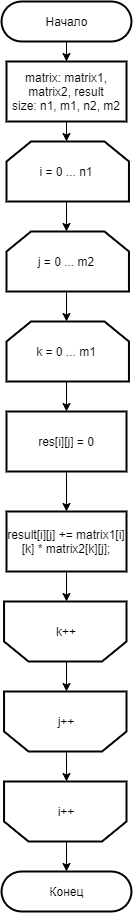
\includegraphics[scale=0.6]{SchemeStand}
        \caption{Классический алгоритм умножения матриц}
        \label{schema:num_1}
    \end{figure}

    \begin{figure}[!htbp]
        \centering
        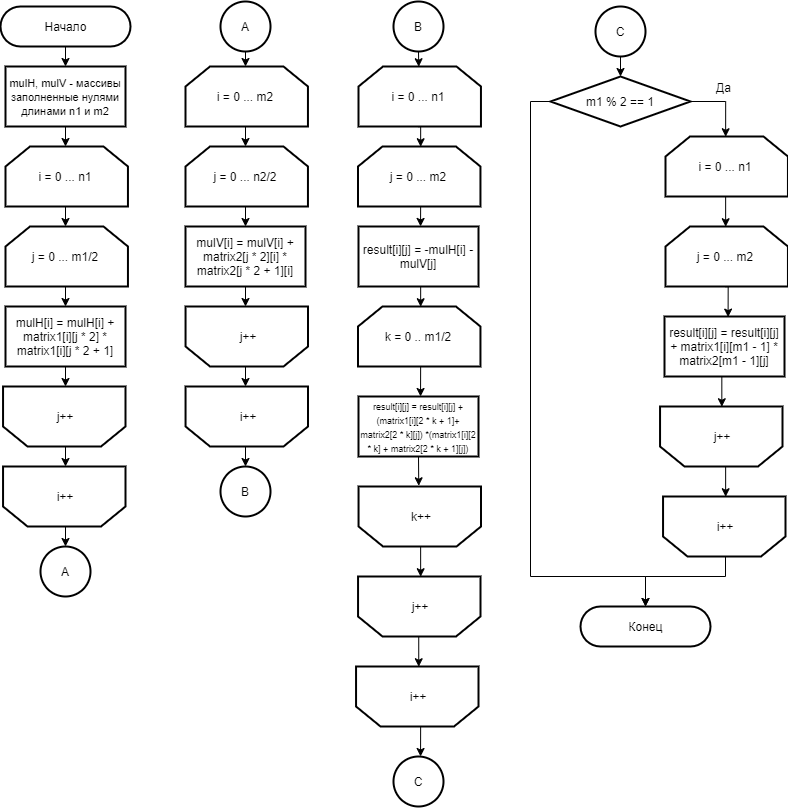
\includegraphics[scale=0.63]{SchemeVin}
        \caption{Алгоритм Винограда}
        \label{schema:num_2}
    \end{figure}

    \begin{figure}[!htbp]
        \centering
        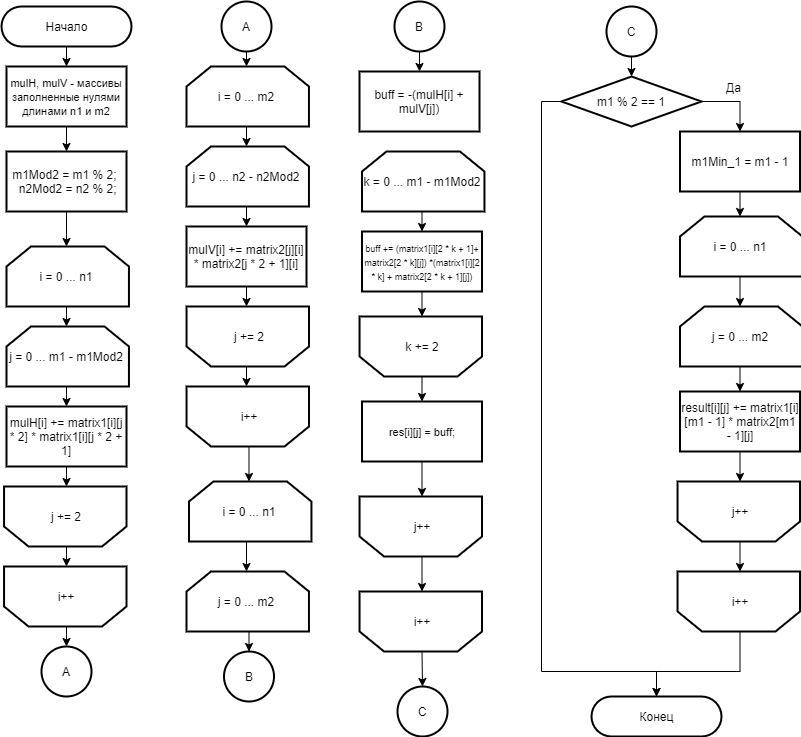
\includegraphics[scale=0.63]{SchemeVinOpt}
        \caption{Алгоритм Винограда с оптимизациями}
        \label{schema:num_3}
    \end{figure}

\newpage
    \section{Трудоёмкость алгоритма}
        Трудоёмкость -- количество работы, которую алгоритм затрачивает на обработку данных.
        Является функцией от длины входов алгоритма и позволяет оценить количество работы.

        Введём модель вычисления трудоёмкости.

        \subsection{Базовые операции}
            Ниже представлены базовые операции, стоимость которых единична:
            \begin{enumerate}
                \item $ =, +, +=, -, -=, *, *=,  /, /=, ++, --, \% $,
                \item $ <, \leqslant, ==, \neq, \geqslant , > $,
                \item $ [ $  $ ] $.
            \end{enumerate}
            
        \subsection{Условный оператор}
            if (условие) \{

                // тело A

            \}

            else \{

                // тело B
            
            \}

            Пусть трудоёмкость тела A равна $ f_A $, а тела B $ f_B $, тогда
            стоимость условного оператора можно найти по формуле (\ref{equation:trud:if}):
            \begin{equation}
                f_{if} = f_\text{условия} + \left\{
                    \begin{matrix}
                    min(f_A, f_B) - \text{лучший случай},\\
                    max(f_A, f_B) - \text{худший случай} 
                    \end{matrix}\right.
                \label{equation:trud:if}
            \end{equation}

        \subsection{Цикл со счётчиком}
            for (int i = 0; i < n; i++) \{

                // тело цикла

            \}
            
            Начальная инициализация цикла (int i = 0) выполняется один раз.
            Условие i < n проверяется перед каждой итерацией цикла и при входе в цикл -- n + 1 операций.
            Тело цикла выполняется ровно n раз.
            Счётчик (i++) выполняется на каждой итерации, перед проверкой условия, т.е. n раз.
            Тогда, если трудоёмкость тела цикла равна $ f $, трудоёмкость всего цикла определяется формулой (\ref{equation:trud:for})

            \begin{equation}
                f_\text{цикла} = 2 + n(2 + f)
                \label{equation:trud:for}
            \end{equation}


\newpage
\subsection{Стандартный алгоритм}
            Найдём трудоёмкость стандартного алгоритма.
            
            $ f_\text{первый цикл} = 2 + N1(2 + f_\text{второй цикл})$  

            $ f_\text{второй цикл} = 2 + M2(2 + f_\text{третий цикл} + 3)$  

            $ f_\text{третий цикл} = 2 + N1(2 + 8)$  

            $ f_\text{Стандартный} = 10N1M2N1 + 7N1M2 +4N1 + 2 \approx 10N1M1N1$

        \subsection{Алгоритм Винограда}
            Найдём трудоёмкость алгоритма Винограда.
            
            $ f_\text{первый цикл} = 2 + N1(2 + \frac{M1}{2}(2 + 12)) = 7N1M1 + 2N1 + 2$
            
            $ f_\text{второй цикл} = 7N2M2 + 2N1 + 2$

            $ f_\text{третий цикл} = 2 + N1(2 + M2(2 + 7 + \frac{M1}{2}(2 + 23))) = 12N1M1M2 + 9N1M2 + 2N1 + 2$

            Условный переход $f_{if} = 2 + \left\{
                \begin{matrix}
                0 - \text{лучший случай},\\
                15N1M2 + 2N1 + 2 - \text{худший случай} 
                \end{matrix}\right.$

            Итого:
            \begin{equation}
                f_\text{Винограда} = 12N1M1N1 + 16N1M2 + 7M1N1 + 6N1 + 6 +
                    \left\{ \begin{matrix}
                    0 - \text{л.с.},\\
                    15N1M2 + 2N1 + 2 - \text{х.с.} 
                    \end{matrix}\right.
            \end{equation}
            $ f_\text{Винограда} \approx 12MNQ $
        \subsection{Оптимизированный алгоритм Винограда}

            Найдём трудоёмкость оптимизированного алгоритма Винограда.
                
            $ f_\text{первый цикл} =\frac{11}{2}(N1M1 + 4N1 + 2)$
            
            $ f_\text{второй цикл} = \frac{11}{2} M2N2+ 4M2 + 2$

            $ f_\text{третий цикл} = \frac{17}{2} N1M2M1 + 9N1M2 + 4N1 + 2$

            Условный переход $f_{if} = 2 + \left\{
                \begin{matrix}
                0 - \text{лучший случай},\\
                10N1M2 + 4N1 + 2 - \text{худший случай} 
                \end{matrix}\right.$

            Итого:
            \begin{equation}
                f_\text{Винограда} = \frac{17}{2}N1M2M1 + \frac{11}{2}N1M1 + \frac{11}{2}M2N2 + 9N1M2 + 8N1 + 4M2 + 6 + 
                    \left\{ \begin{matrix}
                    0 - \text{л.с.},\\
                    10N1M2 + 4N1 + 2 - \text{х.с.} 
                    \end{matrix}\right.
            \end{equation}

\section{Вывод}
В данном разделе были рассмотрены схемы алгоритмов умножения матриц, введена модель оценки трудоемкости алгоритма, были расчитаны трудоемкости алгоритмов в соответсвии с этой моделью. При cхожем коэффициенте при старшем слагаемом в трудоемкости алгоритма Винограда и стандартного, доля долгих операций умножения в алгоритме Винограда меньше.

\chapter{Технологическая часть}
В данном разделе будут выбраны средства реализации ПО, представлен листинг кода
и будет показан метод тестирования.
\section{Средства реализации}
Для реализации программ я выбрал язык программирования C++, так как имею большой опыт работы с ним.
Для замера процессорного времени была использована ассемблерная вставка \cite{link_time}.


\section{Сведения о модулях программы}
Программа состоит из:
\begin{itemize}
	\item main.cpp - главный файл программы, в котором располагается точка входа в программу.
	\item main\_test.cpp - файл с функциями тестирования и замера времени.
	\item util.cpp - файл с функциями для выделения/заполнения/удаления матрицы.
	\item matrix\_multiplication.cs - файл c реализациями 3-х алгоритмов умножения матриц.
\end{itemize}

    \section{Листинг программы}
        Ниже представлены листинги кода поиска растояния Левенштейна: \begin{enumerate}
            \item классический алгоритм (листинг \ref{num_1});
            \item алгоритм Винограда (листинг \ref{num_2});
            \item алгоритм Винограда с оптимизациями (листинг \ref{num_3}).
        \end{enumerate}

\begin{lstlisting}[label=num_1,caption=Классический алгоритма умножения матриц, escapechar=@]
IMatr_t classic_mult_matrix(IMatr_t matr1, int n1, int m1, IMatr_t matr2, int n2, int m2)
{
    IMatr_t res = alloc_matrix(n1, m2);

    for (int i = 0; i < n1; i++)
    {
        for (int j = 0; j < m2; j++)
        {
            res[i][j] = 0;
            for (int k = 0; k < n1; k++)
                res[i][j] += matr1[i][k] * matr2[k][j];
        }
    }

    return res;
}
\end{lstlisting}

\newpage
\begin{lstlisting}[label=num_2,caption=Алгоритма Винограда]
IMatr_t vinograd_mult_matrix(IMatr_t matr1, int n1, int m1, IMatr_t matr2, int n2, int m2)
{
    IMatr_t res = alloc_matrix(n1, m2);

    IArr_t mulH = (IArr_t)calloc(n1, sizeof(int));

    for (int i = 0; i < n1; i++)
    {
        for (int j = 0; j < m1 / 2; j++)
        {
            mulH[i] = mulH[i] + matr1[i][j * 2] * matr1[i][j * 2 + 1];
        }
    }

    IArr_t mulV = (IArr_t)calloc(m2, sizeof(int));

    for (int i = 0; i < m2; i++)
    {
        for (int j = 0; j < n2 / 2; j++)
        {
            mulV[i] = mulV[i] + matr2[j * 2][i] * matr2[j * 2 + 1][i];
        }
    }

    for (int i = 0; i < n1; i++)
    {
        for (int j = 0; j < m2; j++)
        {
            res[i][j] = -mulH[i] - mulV[j];
            for (int k = 0; k < m1 / 2; k++)
            {
                res[i][j] = res[i][j] + (matr1[i][2 * k + 1] + matr2[2 * k][j]) * (matr1[i][2 * k] + matr2[2 * k + 1][j]);
            }
        }
    }

    if (m1 \% 2 == 1)
    {
        for (int i = 0; i < n1; i++)
        {
            for (int j = 0; j < m2; j++)
            {
                res[i][j] = res[i][j] + matr1[i][m1 - 1] * matr2[m1 - 1][j];
            }
        }
    }

    return res;
}
\end{lstlisting}


\begin{lstlisting}[label=num_3,caption=Оптимизированный алгоритм Винограда, escapechar=@]
IMatr_t vinograd_optimized_mult_matrix(IMatr_t matr1, int n1, int m1, IMatr_t matr2, int n2, int m2)
{

    if ((n1 < 1 || m1 < 1 || n2 < 1 || m2 < 1) || m1 != n2)
    {
        return nullptr;
    }

    IMatr_t res = alloc_matrix(n1, m2);

    IArr_t mulH = (IArr_t)calloc(n1, sizeof(int));

    int m1Mod2 = m1 % 2;

    for (int i = 0; i < n1; i++)
    {
        for (int j = 0; j < (m1 - m1Mod2); j += 2)
        {
            mulH[i] += matr1[i][j] * matr1[i][j + 1];
        }
    }

    IArr_t mulV = (IArr_t)calloc(m2, sizeof(int));

    int n2Mod2 = n2 % 2;

    for (int i = 0; i < m2; i++)
    {
        for (int j = 0; j < (n2 - n2Mod2); j += 2)
        {
            mulV[i] += matr2[j][i] * matr2[j + 1][i];
        }
    }

    for (int i = 0; i < n1; i++)
    {
        for (int j = 0; j < m2; j++)
        {
            int buff = -(mulH[i] + mulV[j]);
            for (int k = 0; k < (m1 - m1Mod2); k += 2)
            {
                buff += (matr1[i][k + 1] + matr2[k][j]) * (matr1[i][k] + matr2[k + 1][j]);
            }
            res[i][j] = buff;
        }
    }

    if (m1Mod2 == 1)
    {
        int m1Min_1 = m1 - 1;
        for (int i = 0; i < n1; i++)
        {
            for (int j = 0; j < m2; j++)
            {
                res[i][j] += matr1[i][m1Min_1] * matr2[m1Min_1][j];
            }
        }
    }

    return res;
}
\end{lstlisting}
\subsection{Оптимизация алгоритма Винограда}
В рамках данной лабораторной работы было предложено 3 оптимизации:
\begin{enumerate}
	\item Избавление от деления в условии цикла;
	\item Замена $mulH[i] = mulH[i] + …$ на $mulH[i] += …$ (аналогично для $mulV[i]$);
	
	\begin{lstlisting}[label=some-code,caption=Оптимизации алгоритма Винограда №1 и №2]
	int m1Mod2 = m1 % 2;

	for (int i = 0; i < n1; i++)
	{
		for (int j = 0; j < (m1 - m1Mod2); j += 2)
		{
			mulH[i] += matrix1[i][j] * matrix1[i][j + 1];
		}
	}

	int n2Mod2 = n2 \% 2;
	for (int i = 0; i < m2; i++)
	{
		for (int j = 0; j < (n2 - n2Mod2); j += 2)
		{
			mulV[i] += matrix2[j][i] * matrix2[j + 1][i];
		}
	}
	\end{lstlisting}

	\item Накопление результата в буфер, чтобы не обращаться каждый раз к одной и той же ячейке памяти. Сброс буфера в ячейку матрицы после цикла.
	\begin{lstlisting}[label=some-code,caption=Оптимизации алгоритма Винограда №3]
for (int i = 0; i < n1; i++)
{
	for (int j = 0; j < m2; j++)
	{
		int buff = -(mulH[i] + mulV[j]);
		for (int k = 0; k < (m1 - m1Mod2); k += 2)
		{
			buff += (matrix1[i][k + 1] + matrix2[k][j]) * (matrix1[i][k] + matrix2[k + 1][j]);
		}
		result[i][j] = buff;
	}
}
\end{lstlisting}
\end{enumerate}

\section{Тестирование}
В таблице \ref{table:testing} отображён возможный набор тестов для тестирования методом чёрного ящика.
В столбцах Классический,  Виноград,  Виноград с опт-ей представлены соответсвенно результаты умножения "Матрица 1" и "Матрица 2", полученные классическим алгоритмом, алгоритмом Винограда и оптимизированным алгоритмом Винограда.


\begin{table}[]
            \caption{Таблица тестовых данных}
	    \centering
            \begin{tabular}{|c|c|c|c|c|c|}
            \hline
            № & Матрица 1 & Матрица 2 & \begin{tabular}[c]{@{}c@{}}Классический\\\end{tabular} & \begin{tabular}[c]{@{}c@{}}Виноград\\ \end{tabular} & \begin{tabular}[c]{@{}c@{}}Виноград с опт-ей\\ \end{tabular} \\ \hline
 	1 &  &  & NULL & NULL & NULL\\
	\hline
	2 & 2 & 2 & 4 & 4 & 4 \\
	\hline
	3 & 0 1 & 0 1 & 1 2 & 1 2 & 1 2\\
	& 1 2 & 1 2 & 2 5 & 2 5 & 2 5\\
	\hline
	4 & 0 1 2 & 0 1 2 & 5 8 11 & 5 8 11 &  5  8 11\\
	& 1 2 3 & 1 2 3 & 8 14 20 & 8 14 20 &  8 14 20\\
	& 2 3 4 & 2 3 4 & 11 20 29 & 11 20 29 & 11 20 29\\
	\hline
            \end{tabular}
            \label{table:testing}
\end{table}

\section{Тестирование}
	В данном разделе выбраны средства реализации ПО, представлены листинги кодов 3-х алгоритмов. По итогам тестирования было показано, что алгоритмы работают корректно.

\chapter{Исследовательская часть}
    В данном разделе будут проведены эксперименты для проведения 
    сравнительного анализа алгоритмов по затрачиваемому процессорному 
    времени \cite{link2}.

\section{Сравнительный анализ на основе замеров времени работы алгоритмов}

Был проведен замер времени работы каждой реализации на матрицах разных рамеров.
В таблице \ref{table:time} приняты следующие обозначения:\begin{enumerate}
            \item Classic -- классический алгоритм;
            \item Vinograd -- алгоритм Винограда;
            \item VinogradOpt -- алгоритм Винограда с оптимизацией.
        \end{enumerate}

Графики по таблице изображены на рисунках \ref{graph:graph1}, \ref{graph:graph2}

\begin{table} [h!]
\caption{Время работы реализации алгоритмов  (в тиках)}
	\centering
	\begin{tabular}{|c c c c|} 
 	\hline
	size & Classic & Vinograd & VinogradOpt \\ [0.8ex] 
 	\hline\hline
 	100x100 & 6981488 & 5041345 & 4027075\\
 	\hline
 	101x101 & 7076101 & 5143886 & 4074936\\
 	\hline
 	200x200 & 54394516 & 42259227 & 32604859\\
 	\hline
 	201x201 & 55843226 & 41372159 & 32886685\\
 	\hline
	300x300 & 222039403 & 167047884 & 134266889\\
	\hline
	301x301 & 204466455 & 152396429 & 123611178\\
	\hline
	400x400 & 535629631 & 399587985 & 318084044\\
	\hline
	401x401 & 528259830 & 411047549 & 318868217\\
	\hline
	500x500 & 1082411370 & 793781145 & 628826685\\
	\hline
	501x501 & 1082811261 & 800560090 & 642382560\\
	\hline
	\end{tabular}
	\label{table:time}
\end{table}


\begin{figure}[h!]
\centering
\begin{tikzpicture}
\begin{axis}[
    	axis lines = left,
    	xlabel={Размер (кол-во строк/столбцов)},
    	ylabel={Время (тики)},
	legend pos=north west,
	ymajorgrids=true,
                    height = 0.5\paperheight, 
                    width = 0.75\paperwidth
]



\addplot table [x = b, y = a] { 
	b      a
100 6981488
200 54394516
300 222039403
400 535629631
500 1082411370
};

\addplot table [x = b, y = a] {
	b      a
100 5041345
200 42259227
300 167047884
400 399587985
500 793781145
};

\addplot table [x = b, y = a] { 
	b      a
100 4027075
200 32604859
300 134266889
400 318084044
500 628826685
};



\legend{
                    классический алгоритм,
                    алгоритм Винограда,
                    алгоритм Винограда с оптимизацией
                };

\end{axis}
\end{tikzpicture}
\caption{Сравнение времени работы алгоритмов при четном размере матрицы} 
\label{graph:graph1}
\end{figure}


\begin{figure}[h!]
\centering
\begin{tikzpicture}
\begin{axis}[
    	axis lines = left,
    	xlabel={Размер (кол-во строк/столбцов)},
    	ylabel={Время (тики)},
	legend pos=north west,
	ymajorgrids=true,
                    height = 0.5\paperheight, 
                    width = 0.75\paperwidth
]

\addplot table [x = b, y = a] { 
	b      a
101 7076101
201 55843226
301 204466455
401 528259830
501 1082811261
};

\addplot table [x = b, y = a] {
	b      a
101 5143886
201 41372159
301 152396429
401 411047549
501 800560090
};

\addplot table [x = b, y = a] { 
	b      a
101 4074936
201 32886685
301 123611178
401 318868217
501 642382560
};



\legend{
                    классический алгоритм,
                    алгоритм Винограда,
                    алгоритм Винограда с оптимизацией
                };

\end{axis}
\end{tikzpicture}
\caption{Сравнение времени работы алгоритмов при нечетном размере матрицы}
\label{graph:graph2}
\end{figure}


\section{Вывод}
Самым медленным алгоритмом оказался алгоритм классического умножения матриц, а самым быстрым — оптимизированный алгоритм Винограда. Причем при нечетных размерах матрицы оба алгоритма Винограда работают чуть медленнее, чем при четных размерах.


\chapter*{Заключение}
\addcontentsline{toc}{chapter}{Заключение}
В ходе лабораторной работы были изучены алгоритмы умножения матриц: стандартный, Винограда; составлен оптимизированный алгоритм Винограда

Экспериментально было подтверждено различие во временной эффективности реализаций алгоритма Винограда и классического алгоритма.

В результате исследований я пришел к выводу, что алгоритм Винограда может заметно увеличить скорость нахождения произведения матриц, следовательно более применим в реальных проектах.
 
%далее сам список используевой литературы
\begin{thebibliography}{}
    \bibitem{link_time}  Ассемблерные вставки в AVR-GCC. // [Электронный ресурс]. Режим доступа: http://we.easyelectronics.ru/AVR/assemblernye-vstavki-v-avr-gcc.html, (дата обращения: 03.10.2020).
    \bibitem{link2}  C/C++: как измерять процессорное время. // [Электронный ресурс]. Режим доступа: https://habr.com/ru/post/282301/, (дата обращения: 03.10.2020).
    \bibitem{link3}  Matrix multiplication. // [Электронный ресурс]. Режим доступа: $https://en.wikipedia.org/wiki/Matrix_multiplication$, (дата обращения: 03.10.2020).

\end{thebibliography}

\end{document}